\documentclass{article}
\usepackage[T1]{fontenc}
\usepackage{lmodern}
\usepackage{graphicx}
\usepackage{amsmath,amssymb}
\usepackage[a4paper,margin=2cm]{geometry}
\usepackage[absolute,overlay]{textpos}
\setlength{\TPHorizModule}{1mm}
\setlength{\TPVertModule}{1mm}
\usepackage[indonesian]{babel}
\usepackage{hyperref}
\setlength{\emergencystretch}{2em}
% unit: Halaman 53

\begin{document}

% === Halaman 53 (python/native) ===

53

Sejarah kriptologi pada bangsa Arab 

dapat dibaca pada seri buku Arabic 

Origins of Cryptology yang 

diterbitkan oleh King Faisal Center 

for Research and Islamic Studies, 

Arab Saudi. 

Kriptografi pada Bangsa Arab

Ibn ad-Durayhim bernama lengkap Ali ibn Muhammad ibn Abd 

al Aziz, Tag ad-Din. Dia lahir di Mosul, Irak, pada bulan 

Sya’ban tahun 712 H atau 1312 M. Dia sering berdagang antara 

Kairo dan Damaskus dan ditunjuk sebagai guru di Masjid 

Umayah Damaskus. Dia pindah ke Mesir tahun 760 H/1359 M 

dan dikirim oleh Sultan sebagai duta kepada raja Abyssinia 

(sekarang Etiopia).

% deskripsi: gambar native xref 263
\noindent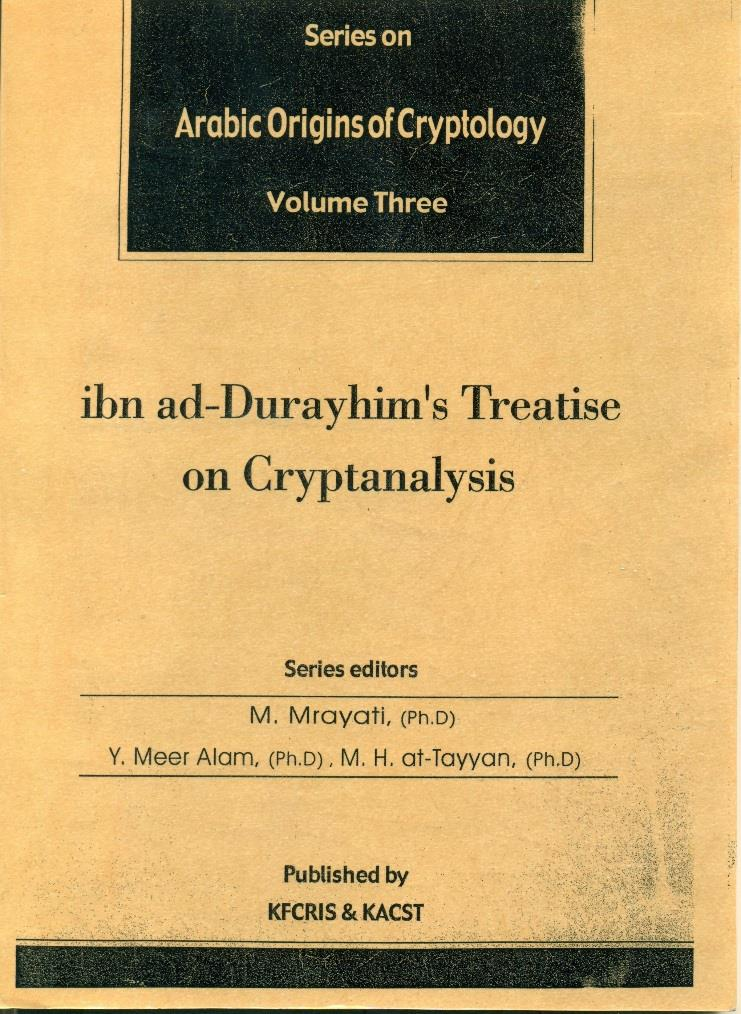
\includegraphics[width=0.85\textwidth]{../../images/python/page_053_img_01.jpeg}

\end{document}
